\section{提案手法}

本研究では,広範な脆弱性情報を効率的に収集し,利用者にとって扱いやすい形式へと変換・管理した上で,脆弱性データベースを構築し,提供する一連のプロセス「データハーベスト」を提案する.
本プロセスは,fetch・extract・db buildの3ステージから構成される.
図\ref{fig:data-harvest}は,各ステージの流れを示す.
fetchステージでは各ベンダーの脆弱性情報を入力とし,vuls-data-rawフォーマットのデータを出力する.
extractステージではvuls-data-rawフォーマットのデータを入力とし,共通スキーマに正規化されたvuls-data-extractedフォーマットのデータを出力する.
db buildステージではvuls-data-extractedフォーマットのデータを入力とし,脆弱性データベースを構築する.
また,データハーベストは継続的インテグレーション(Continuous Integration:CI)上で自動化されており,各ステージが効率的かつ安定的に運用される.
CIを用いた運用により,エラー発生時のパターン蓄積や,データ提供元の仕様変更・フォーマット変更への迅速な対応,障害発生時の復旧,信頼性の高い脆弱性情報の継続的な提供が可能となる.

\begin{figure*}[htbp]
  \begin{center}
    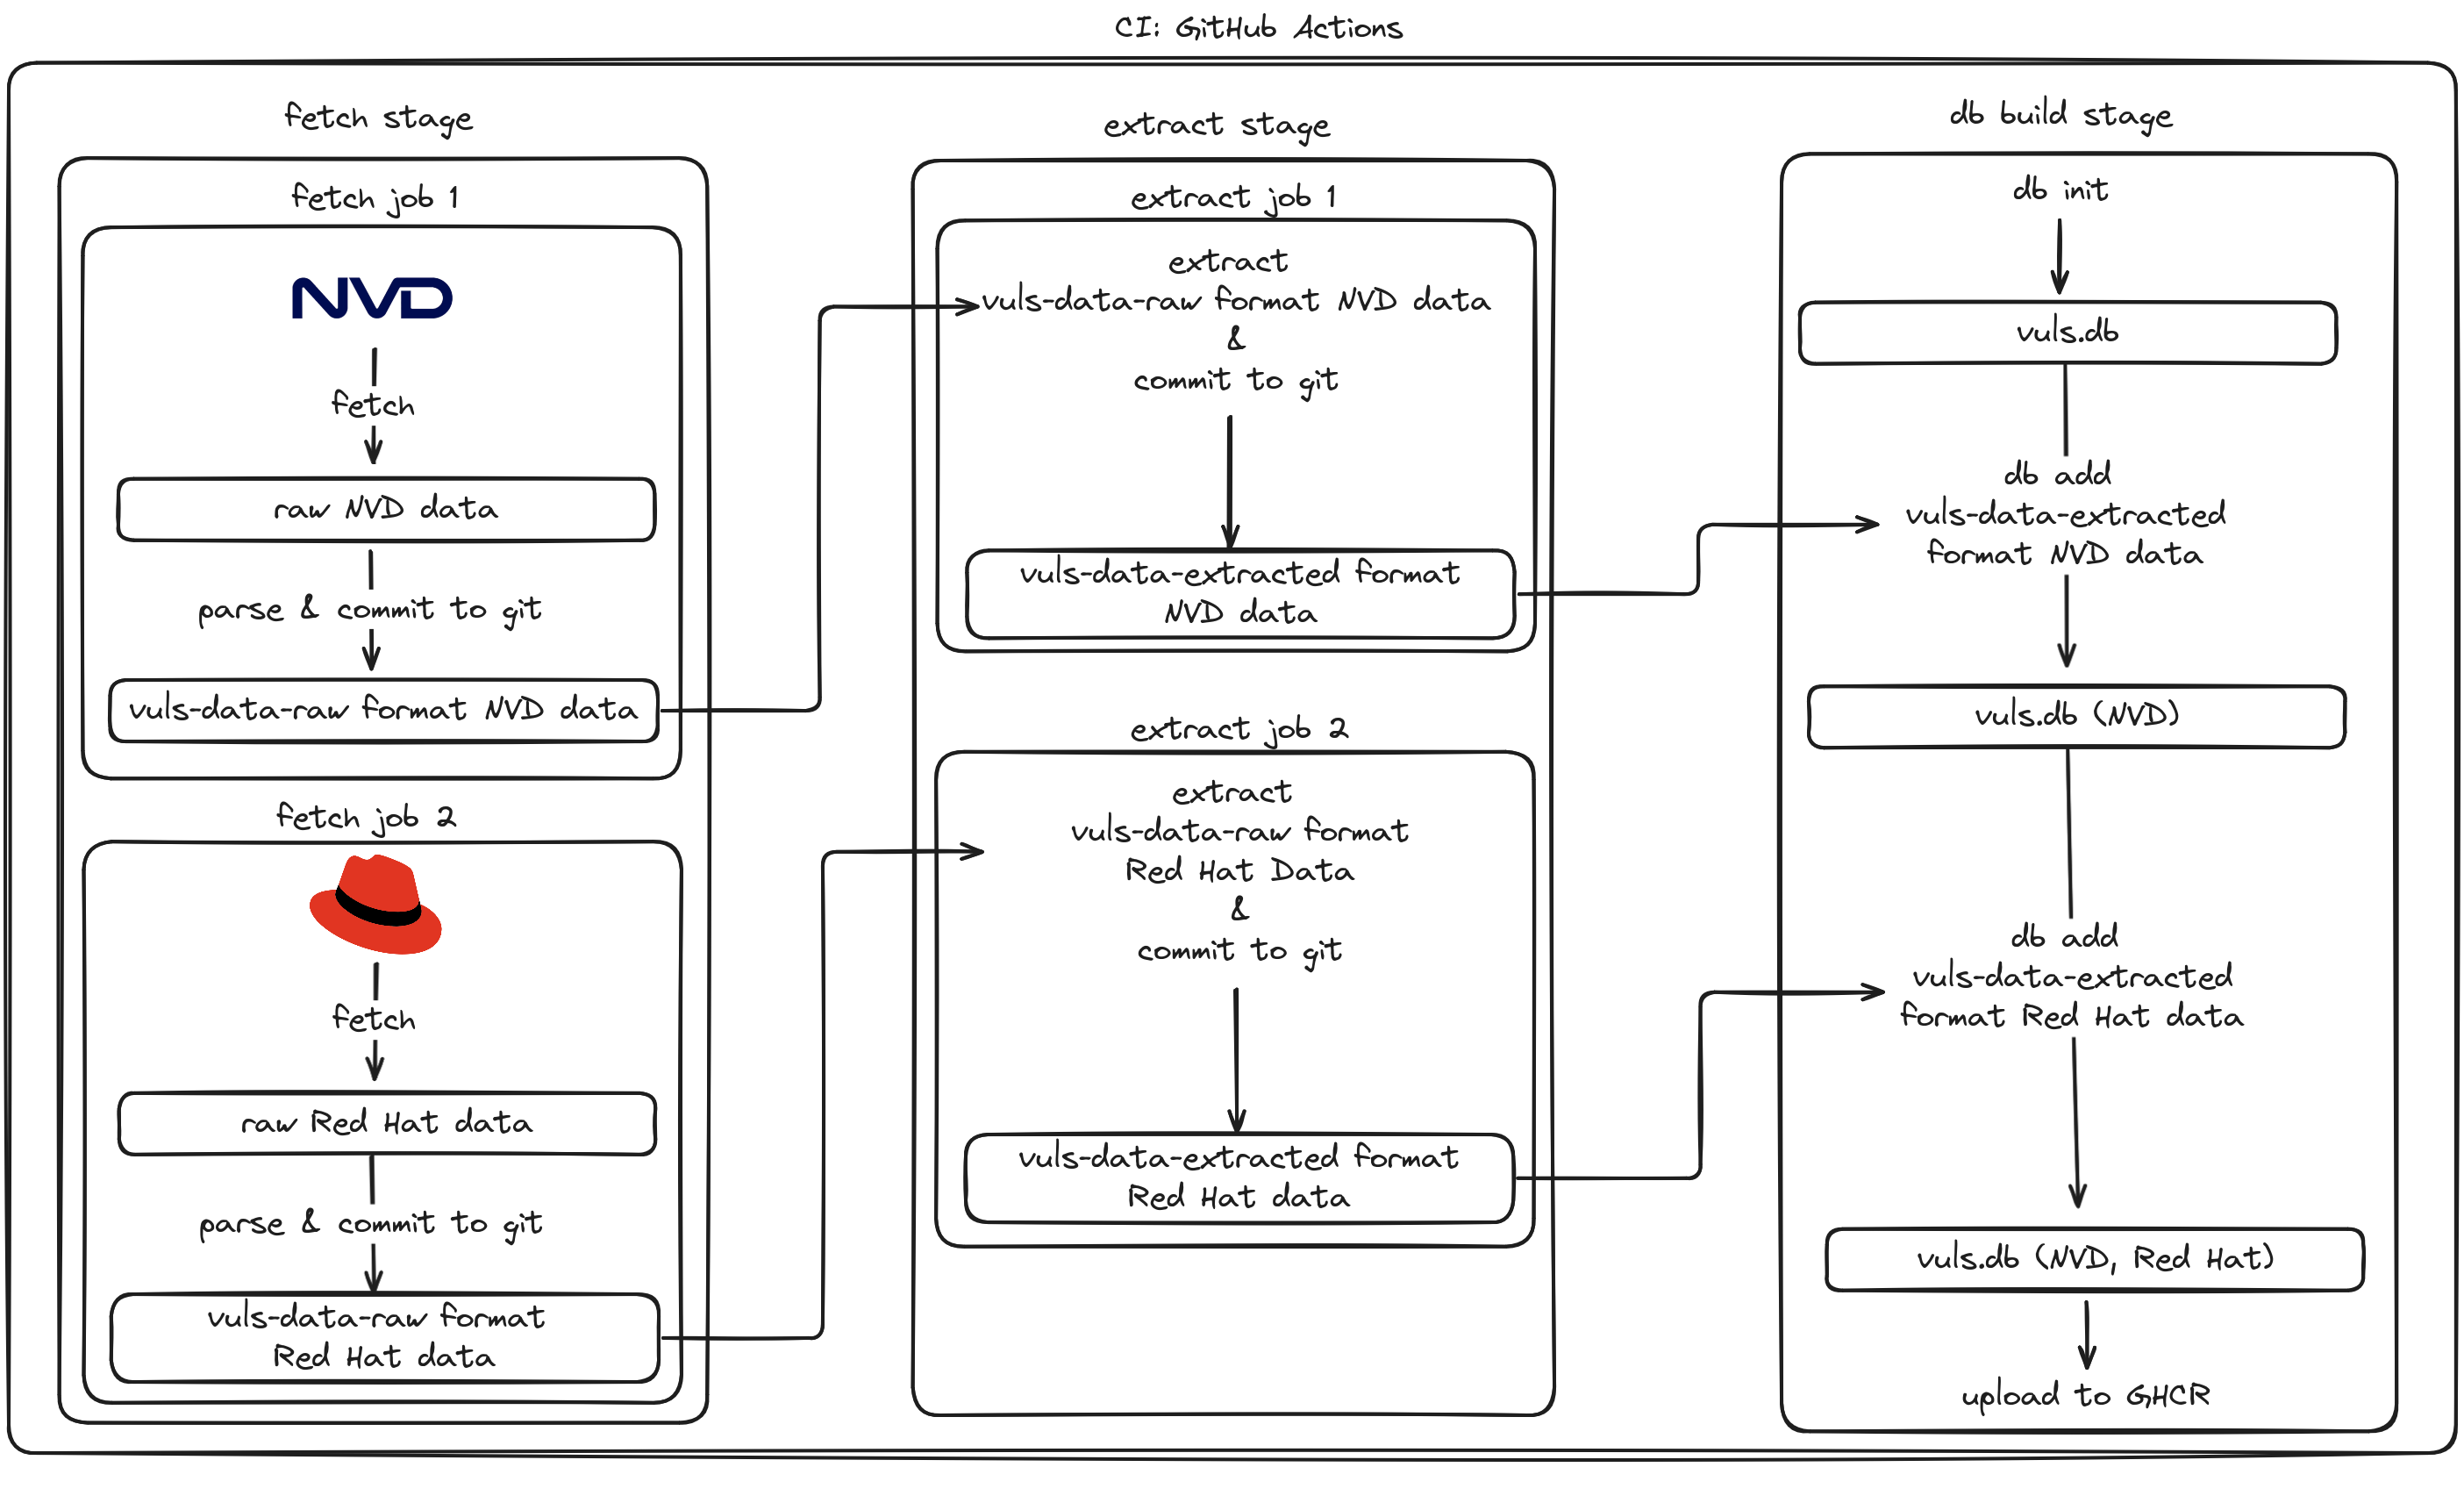
\includegraphics[scale=0.25,angle=90]{./2-methods/data-harvest.png}
    \caption{データハーベスト}
    \label{fig:data-harvest}
  \end{center}
\end{figure*}


\subsection{fetch ステージ(データ収集)}
fetchステージでは,一次データソースから脆弱性情報を収集する.
元のデータの構造をできるだけ保持しつつ,管理しやすい形に整形した状態をvuls-data-rawフォーマットと呼ぶ.
また,保存・管理にはバージョン管理システム(Git)を採用する.
Gitを用いることで,一次データソースの提供元がサーバーダウンして,収集に失敗したとしても,過去に成功した時点のデータを利用できたり,データの差分抽出や履歴管理が容易となり,データの更新や修正の追跡が効率的に行える.

\subsection{extract ステージ(データ変換)}
extractステージでは,fetchステージで収集したvuls-data-rawフォーマットのデータを,共通なデータ構造であるvuls-data-extractedフォーマットへと変換する.
vuls-data-extractedは,vuls-data-rawフォーマットなデータを共通データ構造に正規化したものであり,これにより,多様なデータソースの「方言」を吸収する高度な抽象化レイヤーとして機能し,開発者を各仕様の複雑さから解放する.
extractステージも,fetchステージと同様に変換したデータをGitの管理下に置く.
これにより,vuls-data-rawフォーマットなデータが変更されたことによって,変換が一時的に失敗した場合でも,過去に成功した時点のデータを利用できるため,脆弱性データベースの構築プロセス全体が停止することを防ぐことができる.


\subsection{db build ステージ(データベース構築)}
db buildステージでは,vuls-data-extractedフォーマットのデータを,脆弱性スキャナや脆弱性調査で容易に活用できるような形式でデータベースに格納する.
構築された脆弱性データベースは,GitHub Container Registryを通じて配布され,広範な利用者への提供が実現される.
